\documentclass{article}

\usepackage{multirow}
\usepackage{graphicx}
\usepackage{subcaption}
\usepackage{geometry}
\geometry{margin=.5in}

\begin{document}
\section{Without post processing}
    \begin{figure*}[h!]
        \centering
        \begin{subfigure}[t]{0.5\textwidth}
            \centering
            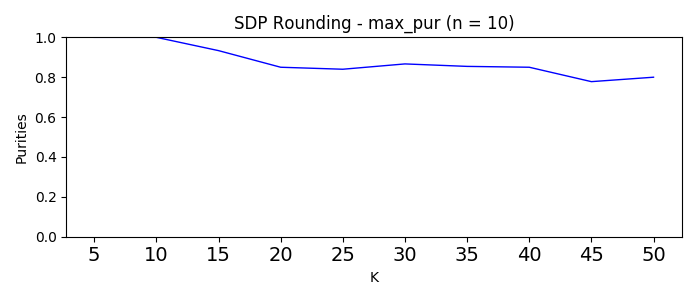
\includegraphics[width=\textwidth]{max_pur_10n_false}
            \caption{}
        \end{subfigure}%
        ~ 
        \begin{subfigure}[t]{0.5\textwidth}
            \centering
            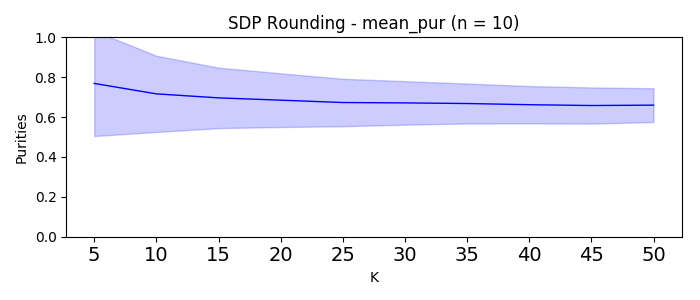
\includegraphics[width=\textwidth]{mean_pur_10n_false}
            \caption{}
        \end{subfigure}
        \begin{subfigure}[t]{0.5\textwidth}
            \centering
            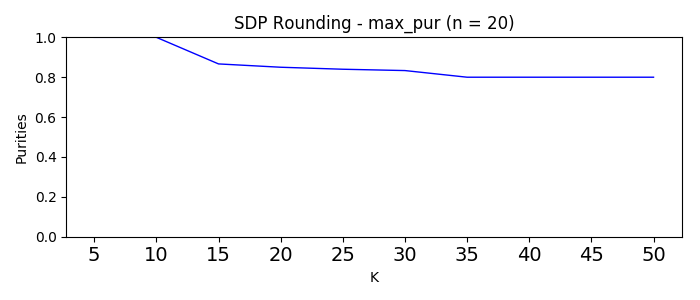
\includegraphics[width=\textwidth]{max_pur_20n_false}
            \caption{}
        \end{subfigure}%
        ~ 
        \begin{subfigure}[t]{0.5\textwidth}
            \centering
            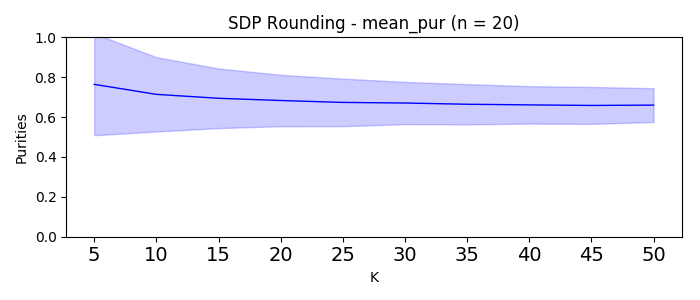
\includegraphics[width=\textwidth]{mean_pur_20n_false}
            \caption{}
        \end{subfigure}
    \end{figure*}
\section{With post processing}
    \begin{figure*}[h!]
        \centering
        \begin{subfigure}[t]{0.5\textwidth}
            \centering
            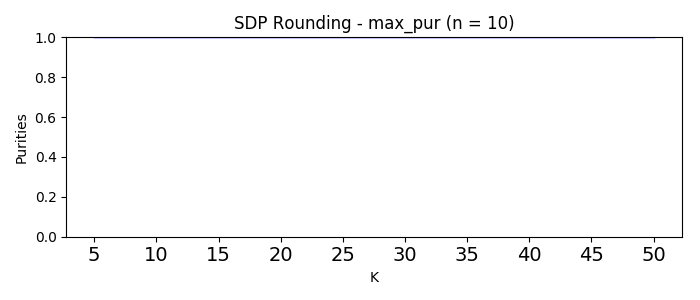
\includegraphics[width=\textwidth]{max_pur_10n_true}
            \caption{}
        \end{subfigure}%
        ~ 
        \begin{subfigure}[t]{0.5\textwidth}
            \centering
            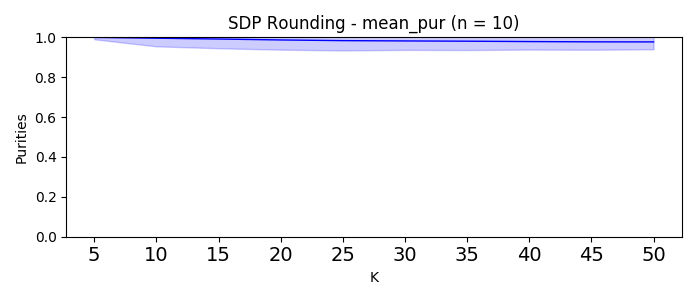
\includegraphics[width=\textwidth]{mean_pur_10n_true}
            \caption{}
        \end{subfigure}
        \begin{subfigure}[t]{0.5\textwidth}
            \centering
            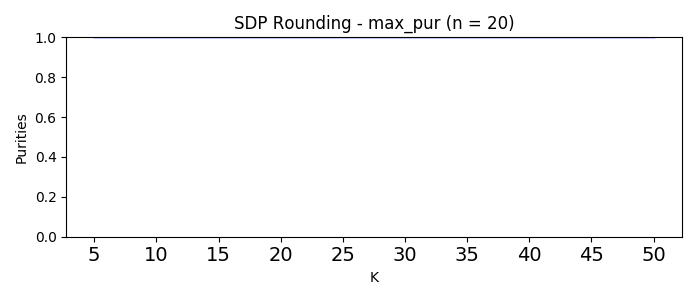
\includegraphics[width=\textwidth]{max_pur_20n_true}
            \caption{}
        \end{subfigure}%
        ~ 
        \begin{subfigure}[t]{0.5\textwidth}
            \centering
            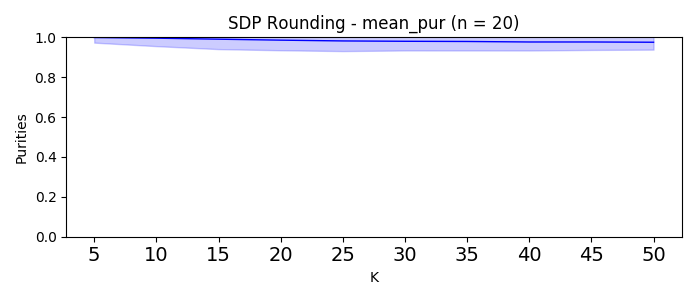
\includegraphics[width=\textwidth]{mean_pur_20n_true}
            \caption{}
        \end{subfigure}
    \end{figure*}
\end{document}
